\chapter{Benchmark}
gfortran installieren:
\begin{lstlisting}[style=Bash]
$ sudo apt-get install gfortran sysfsutils cpufrequtils
\end{lstlisting}
cpu throttling deaktivieren. Wird von atlas verlangt:
\begin{lstlisting}[style=Bash]
$ sudo cpufreq-set -g performance
\end{lstlisting}
ATLAS installieren:
\begin{lstlisting}[style=Bash]
$ ./configure && make
\end{lstlisting}
hpcc downloaden:
\begin{lstlisting}[style=Bash]
$ wget http://icl.cs.utk.edu/projectsfiles/hpcc/download/hpcc-1.4.3.tar.gz
$ tar -xf hpcc-1.4.3.tar.gz
\end{lstlisting}
Make Konfiguration in hpl als Make.Linux ablegen
\begin{lstlisting}[style=Bash]
...
\end{lstlisting}
Kompilieren:
\begin{lstlisting}[style=Bash]
$ make arch=Linux
\end{lstlisting}
Ausführen:
\begin{lstlisting}[style=Bash]
$ mpirun --prefix /shared/tools/openmpi/1.8.4  -n 6 --hostfile /shared/mpi_hosts ./hpcc 
\end{lstlisting}
\section{iozone}
\begin{lstlisting}[style=Bash]
/etc/apt/sources.list non-free
# apt-get update
# apt-get install iozone3
iozone -a -i 0 -g 512M -F /shared/iotmp > bla.txt
$ ./ GenGraph bla.text
\end{lstlisting}
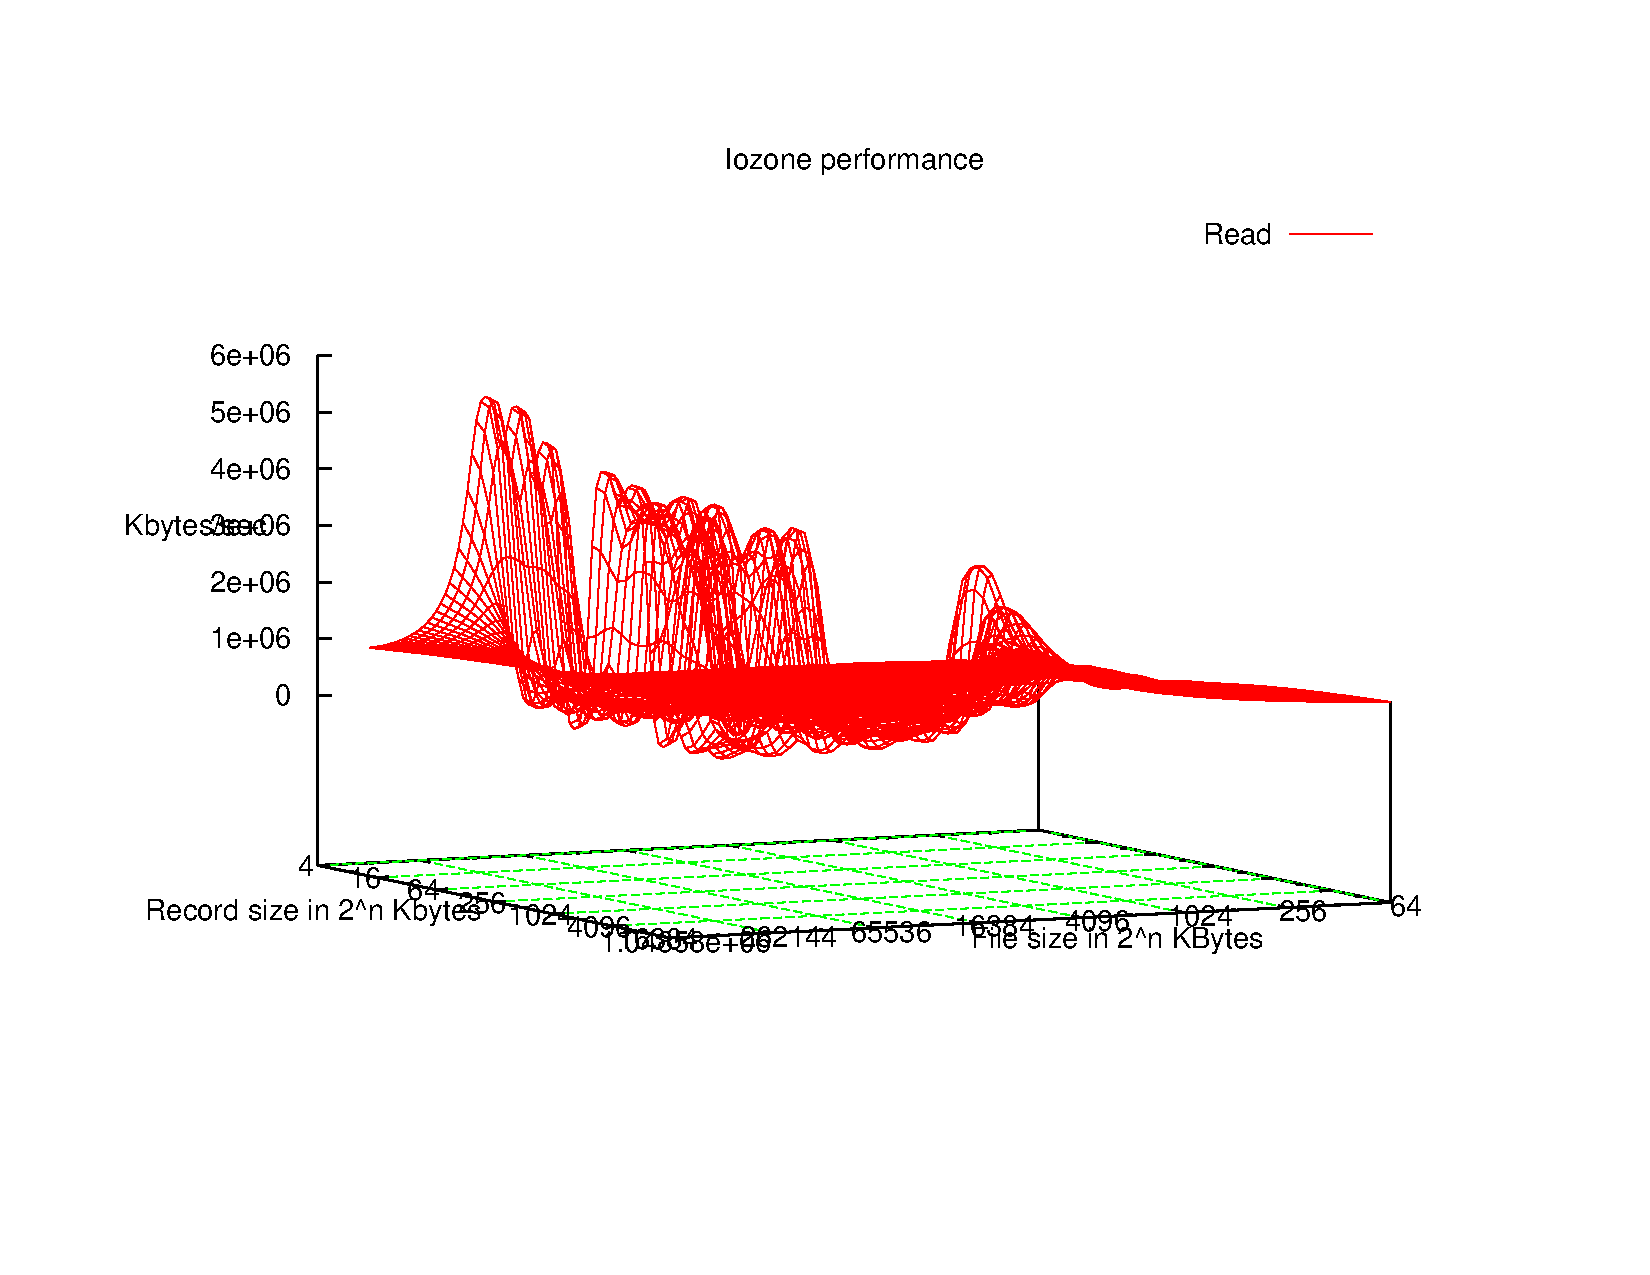
\includegraphics{read.pdf}
